\chapter{Implementation}
\label{ch:impl}
This chapter will describe the implementation of the design application and the WebGL game application, used as a proof of concept for the design presented in Chapter~\ref{ch:design}. 
First the geometry generation stages will be described, as they are common to both applications.
We will then describe the two applications in turn and how they have been implemented.

\section{Geometry Generation}
\label{sec:geomgen}
The geometry Generation phase consists of three phases : 
\begin{enumerate}
	\item Plan Generation
	\item Model Generation
	\item Vertex Generation
\end{enumerate}
These phases and their inputs and outputs are illustrated in Figure~\ref{fig:geomgen}.
Each of these phases are now described in more detail.

\begin{figure}
  \centering
  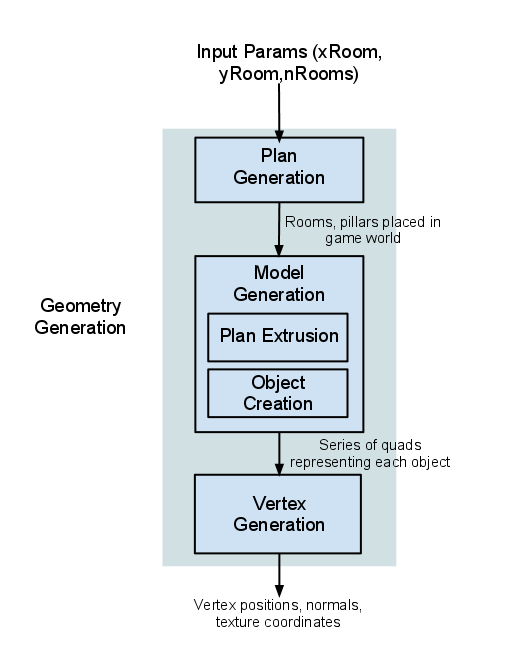
\includegraphics[width=0.7\textwidth]{images/geom_gen}
  \caption{Geometry Generation pipeline}
  \label{fig:geomgen}
\end{figure}

\subsection{Plan Generation}
A lot of time was spent researching different methods for plan generation. 
The plans I focused on were mostly those of office buildings, influenced by Greuter et. al's work on generating entire cityscapes~\cite{greuter2003real}.
As of the time of writing, there is no definitive best way of generating plans of arbitrary buildings.
Martin~\cite{martin2006procedural} created a method for dynamically generating the floor plans of houses.
However the plans generated do not fill a space fully, as is needed in office buildings.
Bradley has written a masters thesis, outlining the potential future areas which can be researched in this area~\cite{bradley2005towards}.
I believe a masters thesis alone could be written on this topic and it there is still much to be done in the area.

For the purposes of this project, I needed a system which would fill a square plan with rooms of a certain pattern.
The pattern chosen was to create rooms along the edges, with rooms in corners extended so as to give them hallway access.
Then rooms in the centre of the plan are generated, in a regular pattern.
This gives the impression that hallways exist in the building.
Once the rooms are placed, windows are added to outward facing walls and doors are added to hallway facing walls.
This is done based on their position within the plan.
Figure~\ref{fig:designapp} shows some generated plans using this system.

Once the rooms are placed, the roof and ceiling are placed to occupy the plan's space.
Pillars are then placed in the corners of rooms with a regular pattern.

\subsection{Model Generation}
The model generation process consists of both plan extrusion and object creation.
Plan extrusion is the process of extruding 2D plans into 3D to create rooms and object creation involves creating other objects such as pillars which cannot simply be extruded.

\subsubsection{Plan Extrusion}
Plan extrusion is done using a few simple ideas.
One is that each room should be represented by a series of rectangles as the walls.
This is depicted in Figure~\ref{fig:planext}.

\begin{figure}
  \centering
  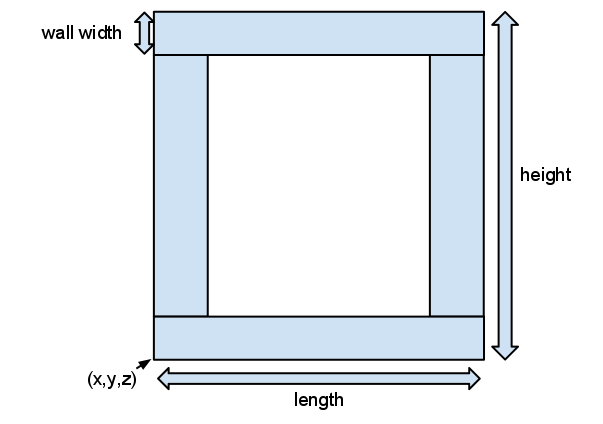
\includegraphics[width=0.6\textwidth]{images/planextrusion}
  \caption{Plan view showing how a room is represented as a set of rectangles}
  \label{fig:planext}
\end{figure}

\begin{figure}
  \centering
  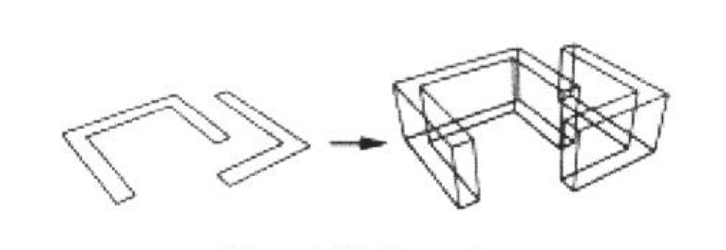
\includegraphics[width=0.5\textwidth]{images/wallextrusion2}
  \caption{How a room is extruded into 3D from a 2D plan.}
  \label{fig:extrusion}
\end{figure}

These rectangles are then extruded into 3D to create cuboids, as is shown in Figure~\ref{fig:extrusion}.
For walls without windows or doors, the extrusion is relatively straightforward.
The result of extruding one wall is 6 quads, which are sent to the vertex generation step along with objects created in the object creation stage.

However when it comes to extruding walls with windows or doors in them the process is somewhat more complicated.
For windows, the process involves creating 4 separate cuboids:
\begin{itemize}
	\item One to the left of the window
	\item One underneath the window
	\item One above the window
	\item One to the right of the window
\end{itemize}
For doors, we omit the cuboid underneath the window, so there is only a cuboid over the door.

Windows and doors are added to a specific wall in a room.
They are given an x and y coordinate to start at on the wall, y being up vertically from the start of the wall, and x horizontally to the right from the start of the wall.
The window/door is then given a width and height.
The resulting cuboids are shown in Figure~\ref{fig:extrudewindow}.
Time did not allow a more general algorithm for creating an arbitrary number of windows so walls are limited to having window or door per wall.

\begin{figure}
  \centering
  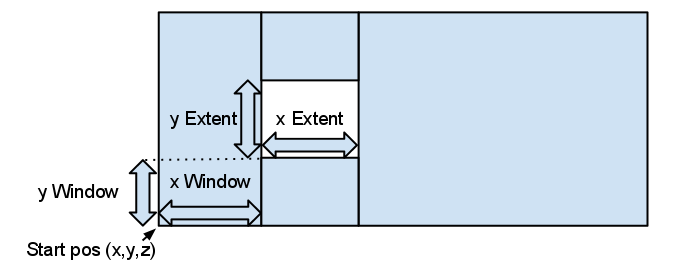
\includegraphics[width=1.0\textwidth]{images/WindowExtrusion}
  \caption{The division of a wall into 4 cuboids to create a window.}
  \label{fig:extrudewindow}
\end{figure}

\subsubsection{Object Creation}
Object creation is the stage that generates all of the non-room objects.
Two of these are the floor and ceiling, which are both represented as simple quads along the x and z axis..
Pillars are the other objects created at this stage.
Pillars are created by progressively creating quads in a circle, by extruding line segments in the plan.
The level of refinement determines the amount of triangles in the resultant model.
The code in Listing~\ref{lst:pillargen} should show how pillars are generated where ``numSlices'' represents the number of quads to generate as part of the process.
The higher this number the more accurate the representation, however it will also use more memory and take longer to generate.

\lstinputlisting[caption=Pillar generation of triangles,label=lst:pillargen]{sourcecode/pillargen.java}

\subsection{Vertex Generation}
Now that we have quads generated using the algorithms described in the previous sections, we can generate the remaining information we need for the WebGL application to display the geometry.
Namely we need a list of triangles, with triangles being represented by a sequence of 3 vertices.
Each vertex needs the following information to be rendered by the WebGL application:
\begin{itemize}
	\item Vertex Position
	\item Normal
	\item Texture coordinate
\end{itemize}
The vertex position is given from the quad, since we can divide a quad with points abcd into two triangles, abc and acd.
The normal is calculated after dividing the quad into two triangles using the cross product as illustrated in Figure~\ref{fig:normal}.
The normal calculation code for a triangle is given in Listing~\ref{lst:normal}.

\lstinputlisting[caption=Normal Calculation for a triangle,label=lst:normal]{sourcecode/normal.java}

The texture coordinates are retrieved using the position on the elevation of the the current vertex on the quad.
The elevation is the view looking along the x or z axes, where y is directly up.
This is illustrated in Figure~\ref{fig:texcoords}.
The code to create the texture coordinates from a quad is shown in Listing~\ref{lst:texcoords}.

\begin{figure}
  \centering
  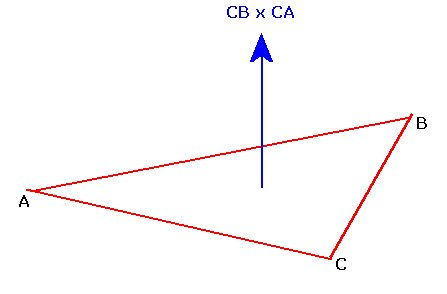
\includegraphics[width=0.4\textwidth]{images/Normal01}
  \caption{Normal calculation for a triangle}
  \label{fig:normal}
\end{figure}

\begin{figure}
  \centering
  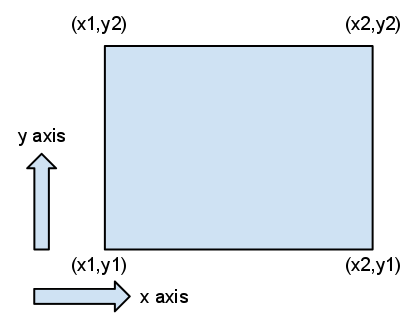
\includegraphics[width=0.4\textwidth]{images/texcoords}
  \caption{Texture Coordinate calculation for a quad. Here the x axis refers to the horizontal axis which could be either the world x or z axis in practice.}
  \label{fig:texcoords}
\end{figure}

\lstinputlisting[caption=Texture Coordinate Generation,label=lst:texcoords]{sourcecode/texcoords.java}

\section{Design Application}
\label{sec:design}
The design application uses the geometry generation phases described in Section~\ref{sec:geomgen} and then outputs the resulting geometry to the user in the form of text files.
Figure~\ref{fig:designpipeline} shows the process in detail.
The design application written in processing, also displays the generated plan to the user.
As shown in the diagram, the final step is to output the vertex information for each model to a file.
The file format is shown in Listing~\ref{lst:fileformat}.
It was designed to be as simple as possible, so that performance could be easily reasoned about.
Each line represents the information for a single vertex.
The first three space-separated values are the position x,y and z coordinates.
The next three space-separated values are the normal's x,y and z coordinates.
The last two space-separated values are the texture coordinates u and v coordinates.
An example file in the format is shown in Listing~\ref{lst:examplefile}, in this case it is to describe a floor model.

\begin{figure}
  \centering
  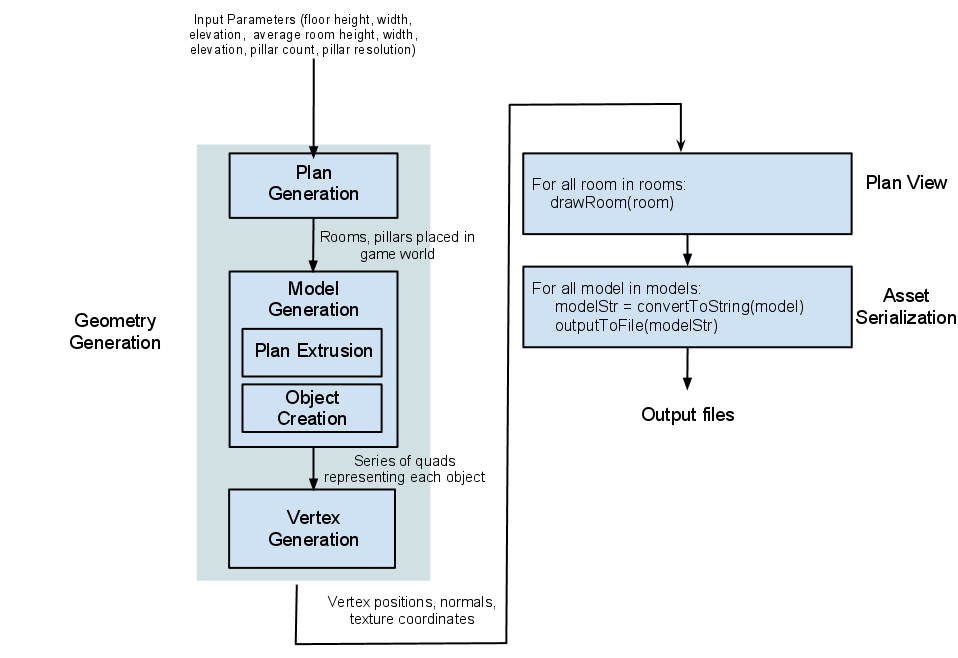
\includegraphics[width=1.0\textwidth]{images/procgl_designprog}
  \caption{Pipeline for the Design Application}
  \label{fig:designpipeline}
\end{figure}

\lstinputlisting[caption=File format for storing models,label=lst:fileformat]{sourcecode/fileformat.java}
\lstinputlisting[caption=Example model file,label=lst:examplefile]{sourcecode/examplefile.java}

\section{WebGL Game Application}
The WebGL game application contains two versions of itself.
Code is reused between these versions to avoid duplication, but they will be described separately to simplify explanation.
One exception is the WebGL drawing code, which is the same for both implementations.
All rendering information is stored in the ModelDrawer and Model classes, so these will firstly be described, before talking about the static and procedural pipelines.

\subsection{ModelDrawer and Model Classes}
The ModelDrawer object basically acts as the frontend for the application for drawing objects in webgl.
It handles the camera movement as well as setting the uniforms which are common to all objects.

The Model object encapsulates a certain type of model, and the model drawer asks it to set the uniforms and attributes which are specific to that type of model.
For instance the pillar model sets the normal attribute which is needed for its vertex shader.

At the end of drawing all of the models to WebGL's rendering context, the ModelDrawer's ``endDraw()'' function is called which will flush the model's drawn which will ensure they are all drawn to the screen before continuing.

\subsection{Static Asset Pipeline}
\label{sec:staticassetimpl}
The static asset pipeline is when the user decides that instead of procedurally generating content, they would like it to be read in from text files.
Figure~\ref{fig:staticasset} shows the flow of program when static assets are chosen.
This is used as the comparison during testing, to investigate how procedural techniques would fare against traditional loading of static models and textures from files.
The shaders used are very simple and simply texture map the texture to the model, without any lighting.
The fragment shader is shown in Listing~\ref{lst:withtexfrag} and the vertex shader is shown in Listing~\ref{lst:withtexvert}.

Model loading is done by loading each model from separate text files, in the format described in Section~\ref{sec:design}.
This is done by going through each line of the file and tokenizing each line, so that each number is a separate token.
We then parse the string token to a float using the java built-in ``Float.parseFloat()'' function.
Listing~\ref{lst:modelloading} shows the function where the parsing of model loading is done.
Once the ArrayList of VertexData is created, we can create vertex, normal and texture coordinate buffers used by WebGL to draw the models.
The methods to do this are in ``AbstractModelLoader.java'' and are shown in Listing~\ref{lst:buffers}.

\lstinputlisting[caption=Static Asset Fragment Shader,label=lst:withtexfrag]{sourcecode/withtexfrag.java}
\lstinputlisting[caption=Static Asset Vertex Shader,label=lst:withtexvert]{sourcecode/withtexvert.java}

\lstinputlisting[caption=Loading in models from files,label=lst:modelloading]{sourcecode/TextModelLoader.java}

\lstinputlisting[caption=Creating WebGL Buffers from VertexData ArrayLists,label=lst:buffers]{sourcecode/buffers.java}

\begin{figure}
  \centering
  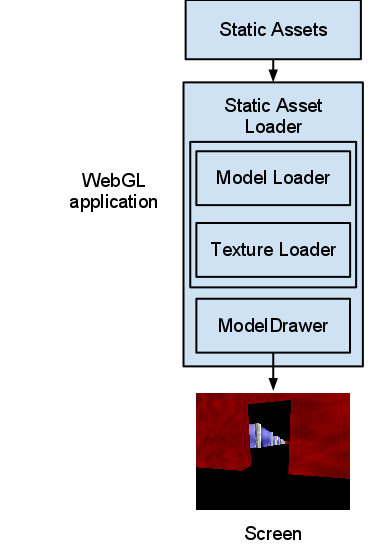
\includegraphics[width=0.4\textwidth]{images/gwtprocstaticassetpipeline}
  \caption{Flow of WebGL Application when used with static assets}
  \label{fig:staticasset}
\end{figure}

\subsection{Procedural Generation Pipeline}
\label{sec:procgen}
The procedural generation pipeline, firstly needs to generate the models used, then it needs to render them with procedurally generated textures.
The generation of models uses the geometry generation phase explained in Section~\ref{sec:geomgen}.
The flow of the program when procedural content is generated on the fly is shown in Figure~\ref{fig:procgenflow}.
The texture generation phases will now be described in Section~\ref{sec:texgen}

\begin{figure}
  \centering
  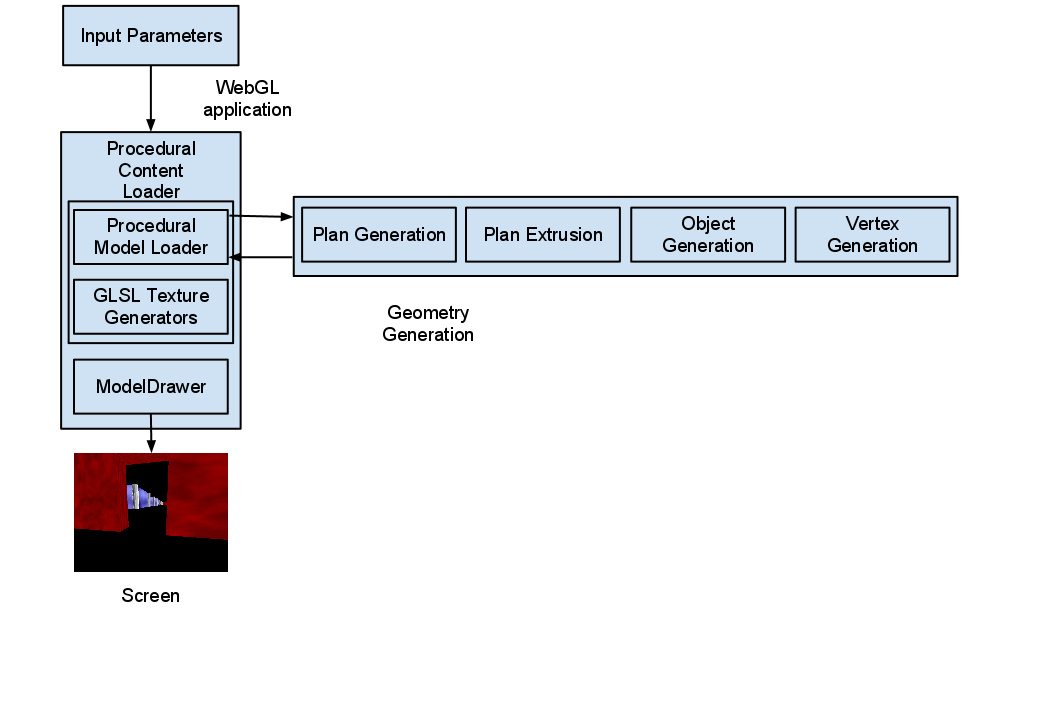
\includegraphics[width=1.0\textwidth]{images/gwtproc_procgenflow}
  \caption{Flow of WebGL Application when the content is procedurally generated}
  \label{fig:procgenflow}
\end{figure}

\section{Texture Generation}
\label{sec:texgen}
Texture Generation is the generation of textures using procedural patterns.
In this way we can create realistic looking materials without physically loading in any texture images.

\subsection{Perlin Noise}
Perlin Noise allows us to generate a wide variety of images base on Ken Perlin's work in 1985~\cite{Perlin:1985:IS:325165.325247}.
Since then perlin noise has found a lot of applications in many areas such as generating heightmaps.
However, one of the original intended uses is to generate materials procedurally.
This project uses an existing GLSL ES shader implmentation of perlin noise, derived from work done by Ashima Arts~\cite{web:webglnoise}.
Ashima's work is based on Gustavson's 2005 work on Simplex noise~\cite{gustavson2005simplex}.
Simplex noise is basically an improvement on perlin noise as it is computationally more efficient and allows for higher dimensionality, up to 5D.

An example of a fragment shader used in this project is shown in Listing~\ref{lst:perlinnoisefrag}, and the corresponding vertex shader is shown in Listing~\ref{lst:perlinnoisevert}.
The shaders shown are to generate the ``sky texture'', and the output of which can be seen in Figure~\ref{fig:sky}

\lstinputlisting[caption=Perlin Noise Fragment Shader,label=lst:perlinnoisefrag]{sourcecode/perlinnoisefrag.java}
\lstinputlisting[caption=Perlin Noise Vertex Shader,label=lst:perlinnoisevert]{sourcecode/perlinnoisevert.java}
\begin{figure}
  \centering
  
\includegraphics[width=0.5\textwidth]{images/sky}
  \caption{Result of applying skybox perlin noise procedural texture}
  \label{fig:sky}
\end{figure}


\subsection{Bump Mapping}
Bump Mapping is achieved entirely within the shaders, by using a distance function to see how far along the texture the point is, and doing lighting calculations based on this.
The effect used is the dimple effect seen in classical-style pillars.
The shader used is a modified version of that used by Rost~\cite{rost2006opengl}, to be more like that of a classical-style pillar.
The fragment shader for bump mapping is shown in Listing~\ref{lst:bumpfrag} and the vertex shader in Listing~\ref{lst:bumpvert}.
A screenshot of the result of these shaders is shown in Figure~\ref{fig:bumpmapping}.

\lstinputlisting[caption=Bump Mapping Fragment Shader,label=lst:bumpfrag]{sourcecode/bumpfrag.java}
\lstinputlisting[caption=Bump Mapping Vertex Shader,label=lst:bumpvert]{sourcecode/bumpvert.java}
\begin{figure}
  \centering
  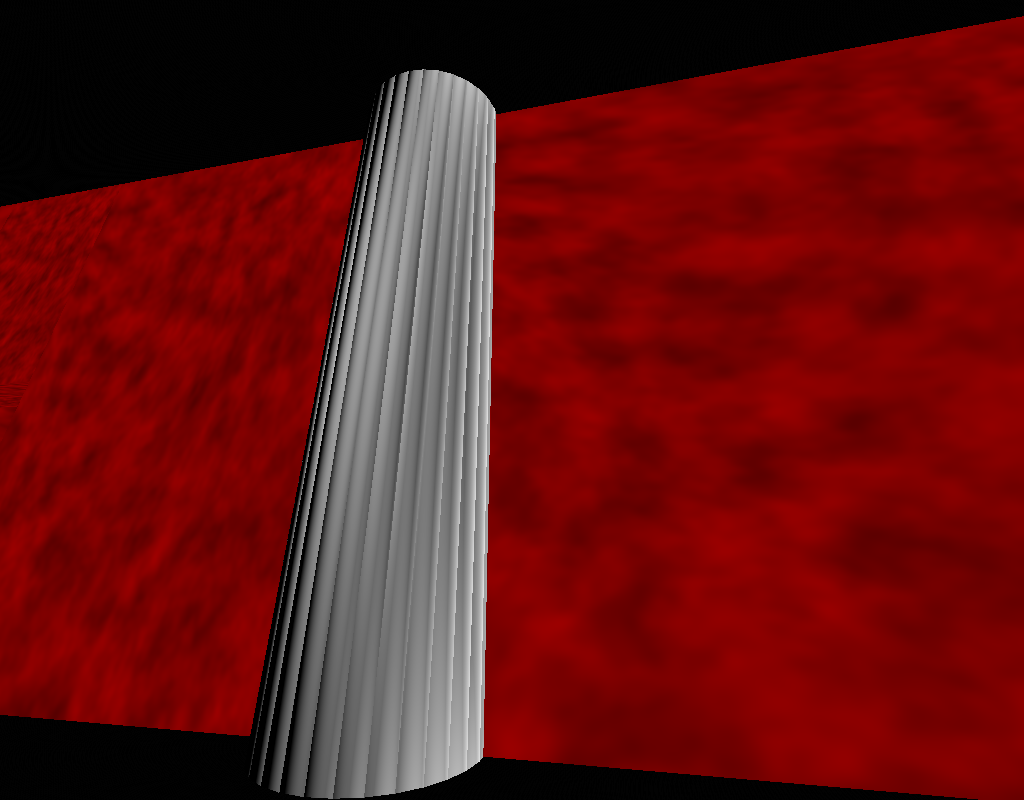
\includegraphics[width=0.5\textwidth]{images/pillar}
  \caption{Procedural bump mapping for a pillar. Notice the classical-style dimples.}
  \label{fig:bumpmapping}
\end{figure}

\subsection{WebGL Limitations}
WebGL has a number of limitations when it comes to procedural texture generation.
Firstly there is no built-in noise() function, so all perlin noise has to be generated manually.
Some OpenGL ES 2.0 extensions are not supported yet which would help in generating textures procedurally.
The main one which would have helped when generating textures was ``OES\_standard\_derivatives''~\cite{web:oesstdder} which was not supported in Firefox 5.0, which was used for development.
This seems to have been rectified with newer releases however, especially with the chromium browser, which seems very up to date with the WebGL Specification~\cite{web:chromium}.
